\batchmode % Do not display issues with package loading
\documentclass[t,12pt]{beamer}

% --------------------------------------------------------------------
% Load packages


%
%   PACKAGES   
%

\usepackage{url}
\usepackage{hyperref}
\usepackage{illcmolthesis}
\usepackage{amsmath}
\usepackage{amssymb}
\usepackage{unicode-math}
\usepackage{verbatim}   % for the comment environment
\usepackage{cleveref}
\usepackage{xcolor}
\usepackage{framed}

% 
%   Minted
% 

\usepackage[outputdir=./out]{minted}

% instruct minted to use our local theorem.py
\newmintinline[leanm]{lean4.py:Lean4Lexer -x}{fontsize=\small}
\newminted[leancode]{lean4.py:Lean4Lexer -x}{fontsize=\small}

% Lean code that does not typecheck/compile
\newminted[badleancode]{lean4.py:Lean4Lexer -x}{%
    fontsize=\small,%
    frame=leftline,%
    framesep=0mm,%
    rulecolor=red%
}

% Disable the red boxed minted will put around "syntax errors" 
\AtBeginEnvironment{minted}{%
  \renewcommand{\fcolorbox}[4][]{#4}}




%   
%   Fonts & coloring
% 

\usepackage[utf8]{inputenc}
\usepackage{newunicodechar}
\usepackage{fontspec}



% switch to a monospace font supporting more Unicode characters
\setmonofont{JetBrains Mono NL Light}
% \setmonofont{Droid Sans Mono}

\newfontfamily{\freemono}{FreeMono}
\newfontfamily{\droidmono}{Droid Sans Mono}
\newfontfamily{\jbmono}{JetBrains Mono NL Light}


% Colors
\definecolor{keywordcolor}{HTML}{008000}
\definecolor{operatorcolor}{HTML}{008000}

% Unicode glyphs

\newcommand\leanoperator[1]{%
\ifx\leanmode\undefined%
#1%
\else%
{\color{operatorcolor} #1}%
\fi%
}
\newcommand\leanmathoperator[1]{\ensuremath{\leanoperator{#1}}} 
\newunicodechar{→}{\leanmathoperator{\rightarrow}}
\newunicodechar{⟹}{\leanmathoperator{\Longrightarrow}}
\newunicodechar{⋅}{\leanmathoperator{\cdot}}

\newunicodechar{α}{{\droidmono α}}
\newunicodechar{β}{{\droidmono β}}
\newunicodechar{γ}{{\droidmono γ}}
\newunicodechar{₁}{\ensuremath{_\text{1}}}
\newunicodechar{₂}{\ensuremath{_\text{2}}}
\newunicodechar{ᵢ}{\ensuremath{_\text{i}}}
\newunicodechar{ⱼ}{\ensuremath{_\text{j}}}
\newunicodechar{ₖ}{\ensuremath{_\text{k}}}
\newunicodechar{ₙ}{\ensuremath{_\text{n}}}
\newunicodechar{ₘ}{\ensuremath{_\text{m}}}
\newunicodechar{₋}{\ensuremath{_\text{-}}}

% 
% \usepackage[GreekAndCoptic]{ucharclasses}
% \setTransitions{GreekAndCoptic}{}{}


% 
%   Spacing & Layout
% 

\usepackage{geometry}

\geometry{
    hmargin=10em
}
\frenchspacing
\setlength{\parskip}{6pt}
\setlength{\parindent}{0pt}



% 
%   Custom environments
% 
\definecolor{shadecolor}{HTML}{F8E0E0}

% definitions
\newenvironment{definition}[1][Definition:]{\begin{trivlist}                         
    \item[\hskip \labelsep {\bfseries #1}]}{\end{trivlist}}
    
% remark    
% \newenvironment{remark}{\begin{trivlist}                         
%   \item[\hskip \labelsep {\bfseries Remark:}]}{\end{trivlist}}



\newenvironment{remark}{%
% \def\FrameCommand{\colorbox{remarkcolor}}%
% \MakeFramed{\advance\hsize-\width \FrameRestore}%
\begin{framed}
\begin{trivlist}
    \item[\hskip \labelsep {\bfseries Remark:}]}%
{%
\end{trivlist}%
\end{framed}
    % \endMakeFramed%
}
    

% todo
\newenvironment{todo}{%
\definecolor{shadecolor}{HTML}{F8E0E0}%
\begin{shaded}%
\begin{trivlist}                         
    \item[\hskip \labelsep {\bfseries Todo:}]}{\end{trivlist}\end{shaded}}

% hidden code    
\newenvironment{leanhidden}{\expandafter\comment}{\expandafter\endcomment}



% 
%   Custom commands
% 

\newcommand\lean[1]{%
\ifx\leanmode\undefined%
\def\leanmode{1}%
\texttt{\small #1}%
\undef\leanmode%%
\else%
\texttt{#1}%
\fi%
}

\newcommand\keyword[1]{{\color{keywordcolor} \textbf{\lean{#1}}}}

\newcommand\inductive{{\keyword{inductive}}}
\newcommand\data{\keyword{data}}
\newcommand\codata{\keyword{codata}}
\newcommand\ldef{\keyword{def}}

\newcommand\Type{\leanm{Type}}
\newcommand\Typen[1]{\leanm{Type #1}}


\newcommand\etal{\emph{et al.}}

% \geometry{
%     hmargin=0
% }

% \usepackage{unicode-math}
% \usepackage{fontspec}
% \usepackage[outdir=./]{minted}
% instruct minted to use our local theorem.py
% \newmintinline[lean]{lean4.py:Lean4Lexer -x}{bgcolor=white}
% \newminted[leancode]{lean4.py:Lean4Lexer -x}{fontsize=\small}

% \usepackage{booktabs}
\usepackage{graphicx}
\usepackage{xcolor}
% \usepackage{tikz}
\usetikzlibrary{calc,trees,positioning,arrows,chains,shapes.geometric,%
    decorations.pathreplacing,decorations.pathmorphing,decorations.markings,shapes,%
    matrix,shapes.symbols,automata,cd,backgrounds, arrows.meta}
\usetikzlibrary{positioning}
\usepackage{color}
\usepackage{mathtools}

% \usepackage{listings}
% \lstset{tabsize=2,showspaces=false,showtabs=false,basicstyle=\ttfamily\mdseries\itshape\normalsize}

\usepackage{algpseudocode}
\usepackage{algorithm}
\usepackage[scr=boondoxo]{mathalpha}
\usepackage[normalem]{ulem}

\usepackage{qtree}

% --------------------------------------------------------------------
% Beamer version theme settings
\usetheme{Frankfurt}
% \usecolortheme{beaver}

% Remove navigation symbols
\setbeamertemplate{navigation symbols}{}

% Better default font
\usepackage{lmodern}
\usepackage[textfont={scriptsize,it}]{caption}
\setbeamerfont{caption}{size=\scriptsize}
\renewcommand*{\familydefault}{\sfdefault}

\usetikzlibrary{overlay-beamer-styles}

% switch to a monospace font supporting more Unicode characters
\setmonofont{FreeMono}
% \font\nullfont=cmr10

% --------------------------------------------------------------------

\def\liketitle#1{%
{\usebeamerfont{frametitle}\usebeamercolor[fg]{frametitle}%
\begin{flushleft}%
\vspace{-\baselineskip}% Cometic correction for space introduced by flushleft
#1\par
\end{flushleft}%
\vspace{-\baselineskip}% Cosmetic correction for space introduced by flushleft
}%
\vspace{0.75\baselineskip}%
}

% --------------------------------------------------------------------
\setbeameroption{hide notes}
%\setbeameroption{show notes}
%\setbeameroption{show notes on second screen}

% --------------------------------------------------------------------
\nonstopmode{} % Include issues with the slides
\beamertemplatenavigationsymbolsempty{}
\setbeamertemplate{navigation symbols}{}

% ====================================================================
% Header settings
\def\lecturename{Lecture}
\title[]{Implementing a definitional (co)datatype package in Lean 4}
\subtitle{Based on Quotients of Polynomial Functors}
\date{}
\author{\textbf{Alex Keizer} \\ Supervised by: \and Jasmin Blanchette \and Benno v.d. Berg}
\subject{}


% ====================================================================
% Main part

% --------------------------------------------------------------------
\batchmode{} % Do not include issues with the package definitions
\begin{document}
\nonstopmode{} % Include issues with the slides



% ====================================================================
\section*{Introduction}

 % --------------------------------------------------------------------
 {
  \begin{frame}[plain]
      \maketitle
  \end{frame}
  \addtocounter{framenumber}{-1}% don't count the title slide.
 }

 % --------------------------------------------------------------------
 {
  \begin{frame}{Lean 4}
      \begin{itemize}
          \item Interactive Theorem Prover / Proof Assistant
          \item Programming Language
                \begin{itemize}
                    \item Functional
                    \item Dependently Typed
                \end{itemize}          
      \end{itemize}

      \bigskip

    \begin{center}
      
\includegraphics[scale=0.22]{lean.png}
    \end{center}

    %   A previous formalization of QPFs exists, but in Lean 3
  \end{frame}
 }


% --------------------------------------------------------------------


\begin{frame}[fragile]{Datatypes are inductive}
    \bigskip
\begin{leancode}
inductive List (α : Type)
  | nil  : List α
  | cons : α → List α → List α
\end{leancode}

\bigskip

\only<2>{
That is,
\begin{itemize}
    \item Let \lean{α} be an arbitrary type, then 
    \item \lean{nil} is a \lean{List α},
    \item If \lean{hd} is an {α} and \lean{tl} is a \lean{List α}, then \\ \lean{cons hd tl} is a \lean{List α},
    \item Nothing else is a \lean{List α}
\end{itemize}
}

% \only<3> {
% Furthermore,
% \begin{itemize}
%     \item \lean{nil ≠ cons hd tl}
%     \item Constructors are injective
% \end{itemize}
% }
\end{frame}



% --------------------------------------------------------------------


\begin{frame}[fragile]{Datatypes are inductive}
    \bigskip
\begin{leancode}
inductive List (α : Type)
  | nil  : List α
  | cons : α → List α → List α
\end{leancode}

\bigskip
Furthermore, the induction principle:
\medskip

\begin{itemize}
    \item Let \lean{P} be a property of lists, if
            \begin{itemize}
                \item \lean{P nil}, and
                \item \lean{P tl} implies \lean{P (cons hd tl)}, for all \lean{hd : α} and \lean{tl : List α},
            \end{itemize}
    \item Then, \lean{P} holds for all lists
\end{itemize}

\end{frame}

    
% --------------------------------------------------------------------


\begin{frame}[fragile]{Codatatypes are coinductive}
    \vfill
\begin{leancode}
codata CoList (α : Type)
  | nil  : CoList α
  | cons : α → CoList α → CoList α
\end{leancode}

\vfill

     
\end{frame}
    
% --------------------------------------------------------------------


\begin{frame}[fragile]{Coinductive Trees}
    \vfill
\begin{leancode}
codata CoTree (α : Type)
  | node : α → CoList (CoTree α) → CoTree α 
\end{leancode}

\medskip

\pause

{
    \hfill
    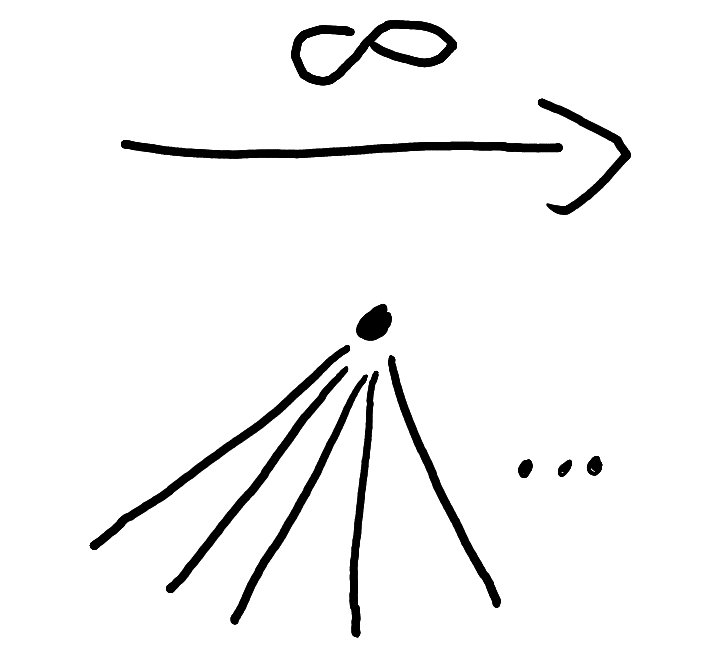
\includegraphics[scale=0.1]{tree_inf_wide.png}
    \hspace*{2.6cm}
    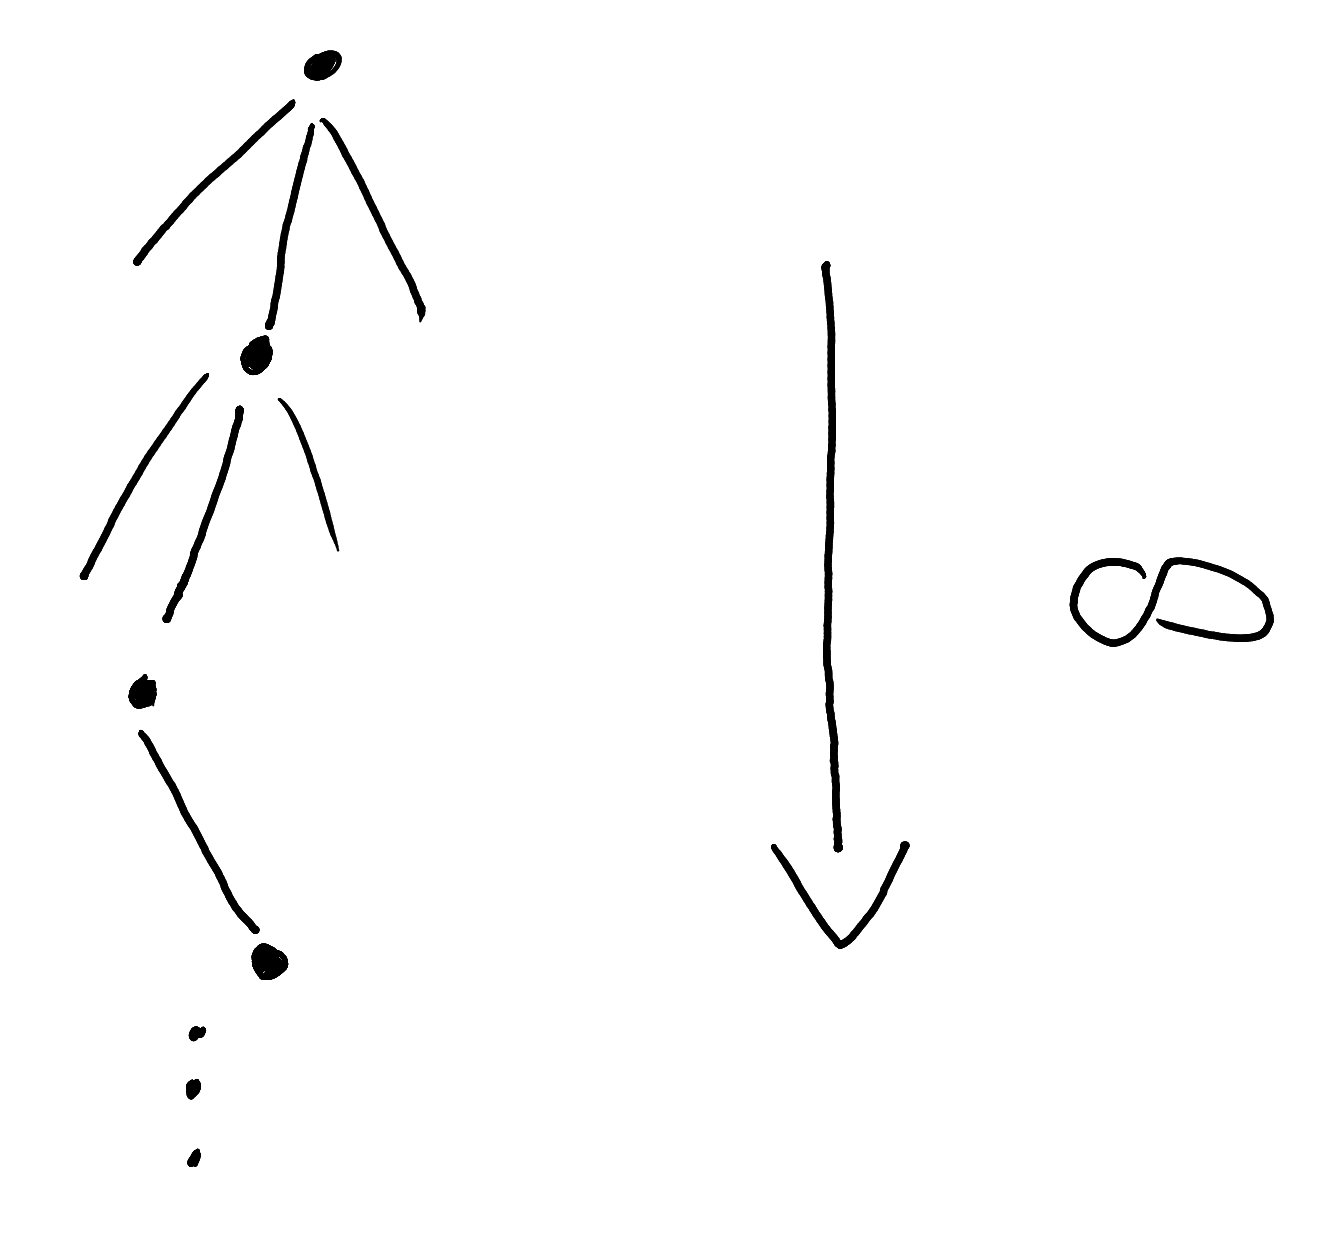
\includegraphics[scale=0.07]{tree_inf_deep.png}    
    \hfill
}



     
\end{frame}
    
% --------------------------------------------------------------------


\begin{frame}[fragile]{Coinductive Trees}
    \vfill
\begin{leancode}
data CoTree2 (α : Type)
  | node : α → CoList (CoTree2 α) → CoTree2 α
\end{leancode}

\medskip

{
    \hfill
    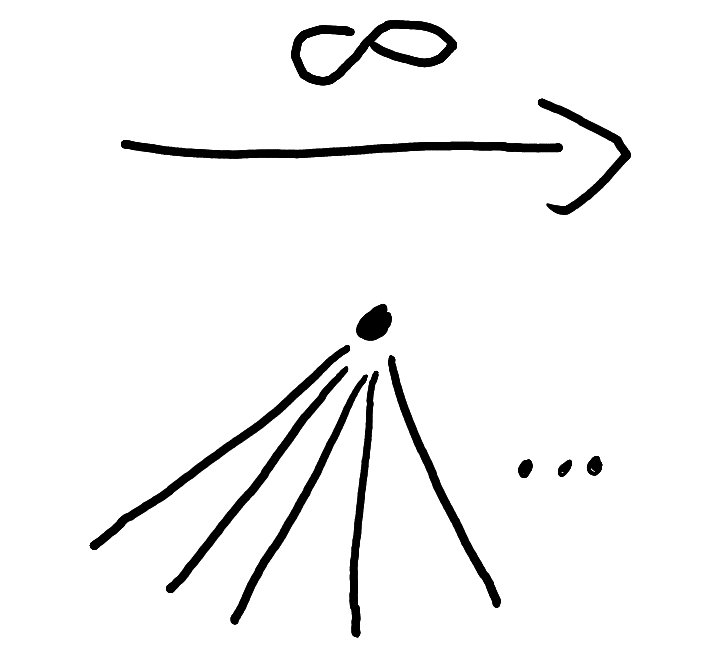
\includegraphics[scale=0.1]{tree_inf_wide.png}
    \hspace*{2.6cm}
    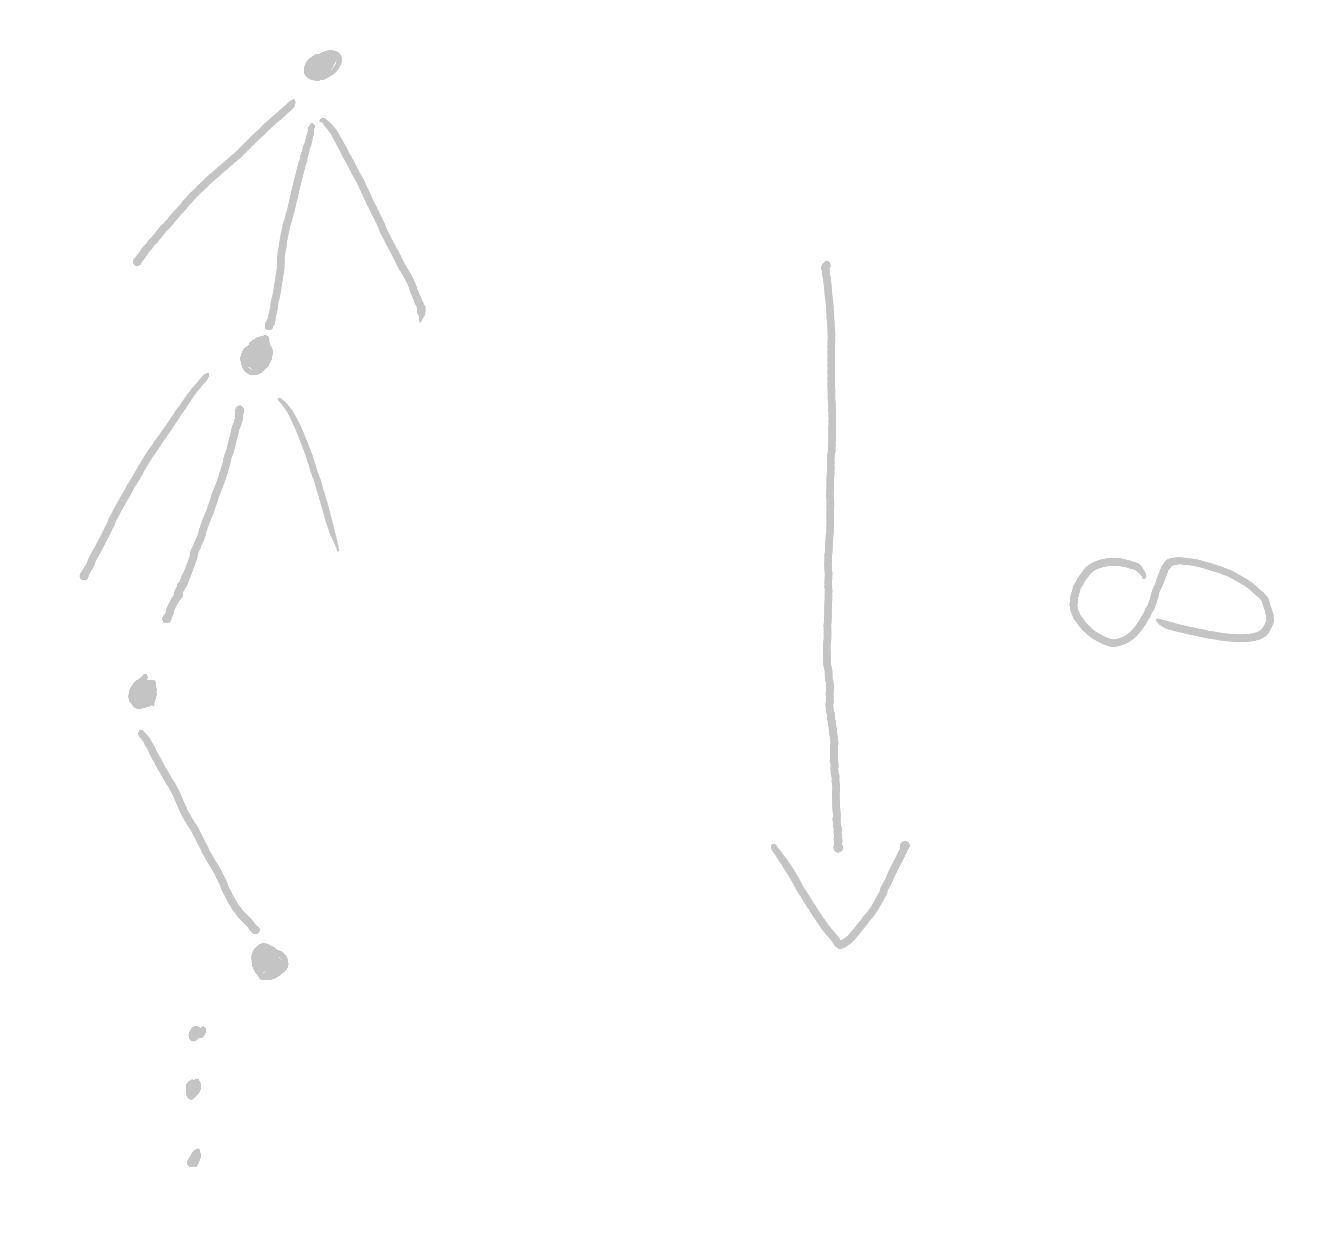
\includegraphics[scale=0.07]{tree_inf_deep_grey.png}    
    \hfill
}



     
\end{frame}
    
% --------------------------------------------------------------------


\begin{frame}[fragile]{Coinductive Trees}
    \vfill
\begin{leancode}
codata CoTree3 (α : Type)
  | node : α → List (CoTree3 α) → CoTree3 α
\end{leancode}

\medskip

{
    \hfill
    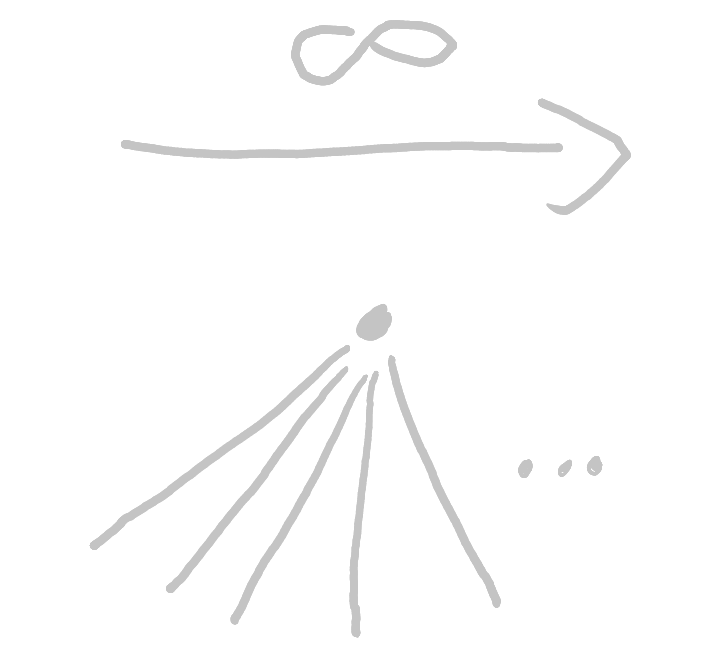
\includegraphics[scale=0.1]{tree_inf_wide_grey.png}
    \hspace*{2.6cm}
    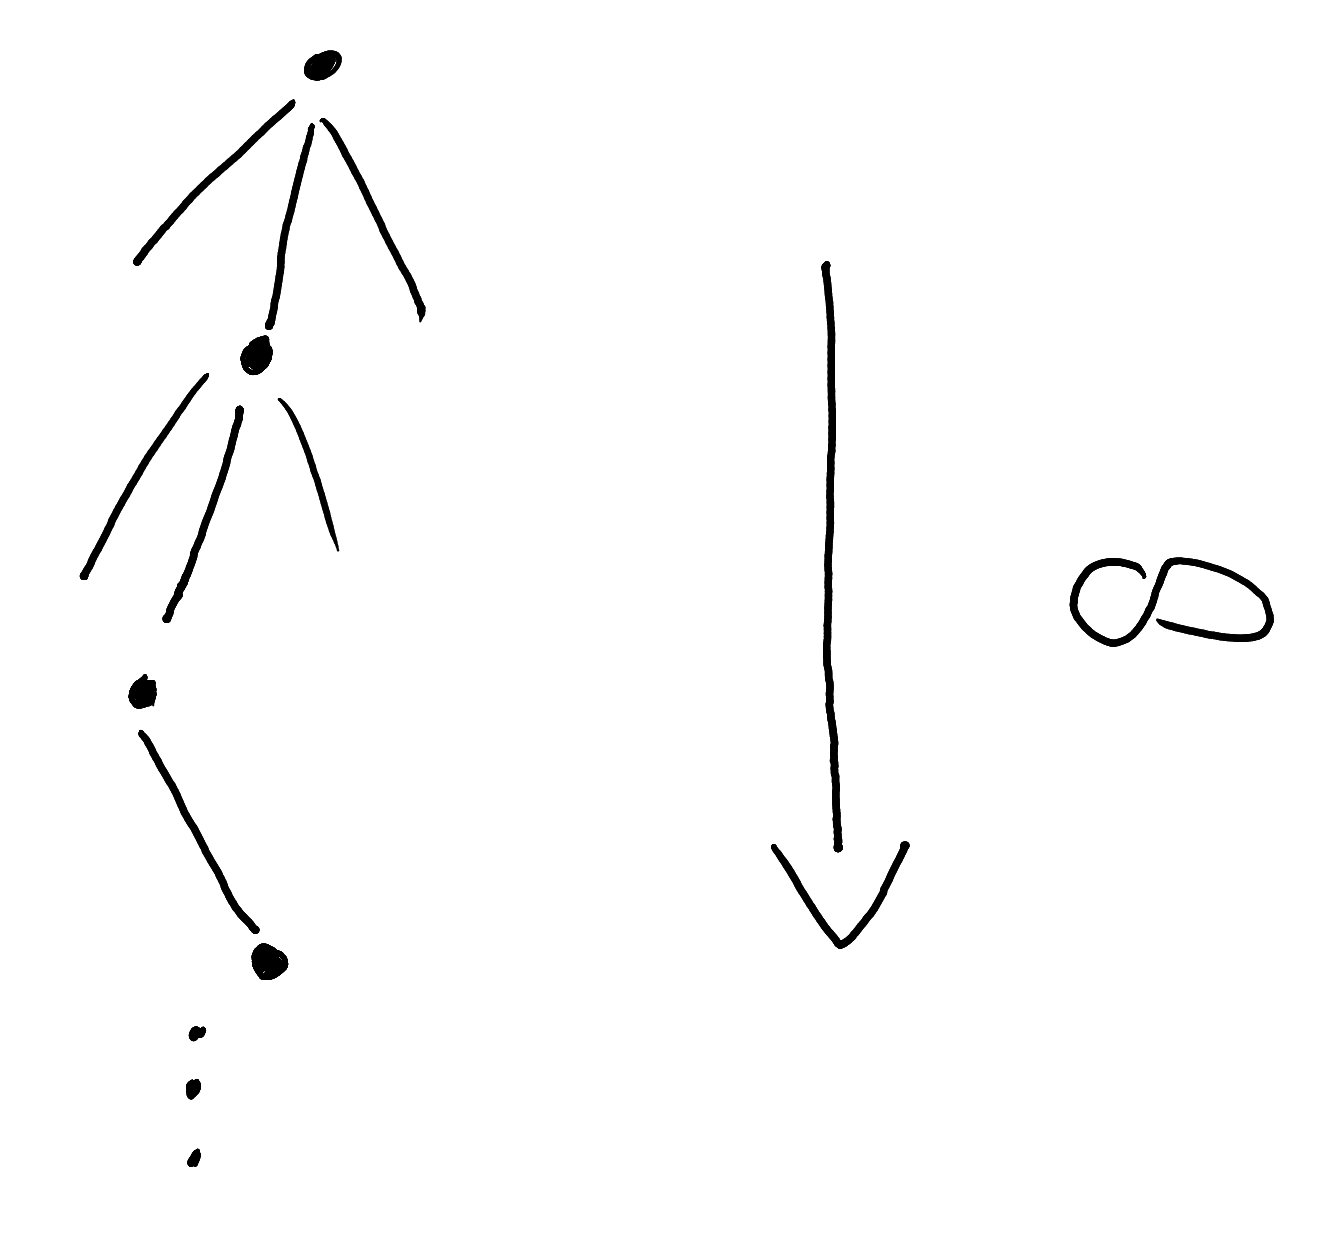
\includegraphics[scale=0.07]{tree_inf_deep.png}    
    \hfill
}



     
\end{frame}
    
% --------------------------------------------------------------------

\begin{frame}{Overview}
    \begin{itemize}
        \setlength{\itemsep}{\fill}

        \item Porting existing building blocks from Lean 3 to Lean 4\footnote{J. Avigad, M. Carneiro, and S. Hudon, “Data Types as Quotients of Polynomial Functors,”
        in \emph{ITP 2019}, vol. 141 of \emph{LIPIcs}}

        \item Enhancing those building blocks
        
        \item Designing a procedure to compile definitional specifications into these building blocks
        
        \item Implementing proof-of-concept \data{} and \codata{} commands
    \end{itemize}

    \vfill
     
\end{frame}





% ====================================================================
\section*{The Procedure}


% --------------------------------------------------------------------

% \begin{frame}[fragile]{Sums and Products}

%     \vfill

%     \begin{center}
%     \begin{leancode}
% inductive Sum (α β : Type)        
%   | inl : α → Sum α β
%   | inr : β → Sum α β
%     \end{leancode}

%     \vfill

%     \begin{leancode}
% inductive Prod (α β : Type)        
%   | mk : α → β → Sum α β
%     \end{leancode}

        
% \end{center}

%     \vfill

% \end{frame}

% --------------------------------------------------------------------

% \begin{frame}{Polynomial Functor}    
%     \vfill
%     A polynomial functor is built up from (finite) sums, products and function spaces (\lean{α → β})
%     \vfill
% \end{frame}

% \begin{frame}{Polynomial Functor}    

%     \vfill

%     \begin{definition}
%         Let $A$ be a type, and $B_a$ an $n$-tuple of types, for every $a : A$.
%         These define an $n$-ary polynomial functor
%         \[
%             P(X_0, \ldots, X_{n-1}) = \sum_{a \mathrel{:} A} B_{a} ⟹ X
%         \]
%         Where $B_{a} ⟹ X$ is short an $n$-tuple of functions
%         \[
%             (B_{a,0} → X_0) × \ldots × (B_{a,n-1} → X_{n-1})
%         \]
%     \end{definition}

%     \vfill
    
% \end{frame}



% --------------------------------------------------------------------



\begin{frame}{Polynomial Functor}

    \vfill

    A polynomial functor $P$ is defined by,
    \begin{itemize}
        \item a type $A$, and
        \item for each $a : A$ a type $B_{a}$
    \end{itemize}

    \vfill

    \[
        P(X) = \sum_{a : A} B_a → X
    \]

    \vfill

    Elements of $P(X)$ are pairs $⟨a,f⟩$ where
    \begin{itemize}
        \item $a : A$ is a \emph{shape}, and
        \item $f : B_a → X$ the \emph{contents}
    \end{itemize}


    \vfill
    
\end{frame}

% --------------------------------------------------------------------


\begin{frame}[fragile]{Option}
    \vfill
    \begin{leancode}
inductive Option (α : Type)
  | none : Option α
  | some : α → Option α        
    \end{leancode}

    \vfill
    \pause


    \begin{tabular}{ll}
        \lean{A := \{ none, some \}}        & \leanm{-- 2 inhabitants}  \\
        \pause
        \lean{B$_{\lean{none}}$ := Empty}   & \leanm{-- 0 inhabitants}  \\
        \lean{B$_{\lean{some}}$ := Unit}    & \leanm{-- 1 inhabitant}    \\    
    \end{tabular}

    \vfill

\end{frame}


% --------------------------------------------------------------------


\begin{frame}[fragile]{Pairs}
    \vfill

    \begin{leancode}
inductive Pair (α : Type)
  | mk : α → α → Option α        
    \end{leancode}

    \vfill
    \pause


    \begin{tabular}{ll}
        \lean{A := \{ mk \}}                & \leanm{-- 1 inhabitant}  \\
        \lean{B$_{\lean{mk}}$ := Fin 2}     & \leanm{-- 2 inhabitants}  \\
    \end{tabular}
    
    \vfill 
    \lean{Fin n} has exactly $n$ inhabitants

\end{frame}


% --------------------------------------------------------------------


\begin{frame}[fragile]{Sum}

    \vfill

\begin{leancode}
inductive Sum (α β : Type)        
  | inl : α → Sum α β
  | inr : β → Sum α β
\end{leancode}

\vfill
\end{frame}

% --------------------------------------------------------------------

\begin{frame}{Polynomial Functor (2 arguments)}

    \vfill

    A \textbf{binary} polynomial functor $P$ is defined by,
    \begin{itemize}
        \item a type $A$, and
        \item for each $a : A$, types \textbf{$\mathbf{B^0_{a}}$ and $\mathbf{B^1_a}$}
    \end{itemize}

    \vfill

    \[
        P(X_0, X_1) = \sum_{a : A} \left( B^0_a → X_0  ×  B^1_a → X_1 \right)
    \]

    \vfill

    Elements of $P(X_0, X_1)$ are \textbf{triples} $⟨a, f_0, f_1⟩$ where
    \begin{itemize}
        \item $a : A$ is a \emph{shape}, and
        \item $f_0 : B^0_a → X_0$ the \emph{contents} for $X_0$, and
        \item $f_1 : B^1_a → X_1$ the \emph{contents} for $X_1$, and
    \end{itemize}


    \vfill
    
\end{frame}

% --------------------------------------------------------------------


\begin{frame}[fragile]{Sum}

    \vfill

\begin{leancode}
inductive Sum (α β : Type)        
  | inl : α → Sum α β
  | inr : β → Sum α β
\end{leancode}

\vfill

\only<1-2>{
    \begin{center}
\begin{tabular}{ll}
    \lean{A := \{ inl, inr \}}  &  \leanm{-- 2 inhabitants}    \\
\end{tabular}
\end{center}
}

\only<2>{
    \medskip
    \begin{center}
        \begin{tabular}{lcc}
                & \lean{α}  & \lean{β} \\ \hline
    \lean{inl}  & 1         & 0 \\
    \lean{inr}  & 0         & 1 \\
        \end{tabular}
    \end{center}
}
\only<3>{
    \begin{center}
\begin{tabular}{ll}
    \lean{A := \{ inl, inr \}}  &  \leanm{-- 2 inhabitants}    \\
    \lean{B$^0_{\lean{inl}}$ := Fin 1} & \lean{B$^1_{\lean{inl}}$ := Fin 0}  \\
    \lean{B$^0_{\lean{inr}}$ := Fin 0} & \lean{B$^1_{\lean{inr}}$ := Fin 1}  \\
\end{tabular}
\end{center}
}


\vfill
    
\end{frame}


% --------------------------------------------------------------------





% \begin{frame}[fragile]{Shape Types}

%     \begin{definition}
%         A shape type is one where the type of each constructor argument is just an instance of a type parameter
%     \end{definition}

%     \pause{}

%     \vfill

%     That is, the type definition

%     \begin{itemize}
%         \item must be non-recursive, and
%         \item may not mention other types,
%     \end{itemize}

% \end{frame}




% --------------------------------------------------------------------


\begin{frame}[fragile]{Recursive Types}

\vfill

    \begin{leancode}
data List (α : Type)
  | nil : List α
  | cons : α → List α → List α
    \end{leancode}

    \vfill
    
\end{frame}

\begin{frame}[fragile]{Recursive Types}

\vfill

    \begin{leancode}
inductive ListShape (α ρ : Type)
  | nil : ListShape α
  | cons : α → ρ → ListShape α
    \end{leancode}

    \vfill

    \pause{}

    \only<-3> {
    \begin{tabular}{rclr}
        \lean{List α} & \lean{=} & \lean{ListShape α (List α)} & \emph{(fixpoint)} \\
        \pause
        \lean{CoList α} & \lean{=} & \lean{ListShape α (CoList α)} & \emph{(cofixpoint)} \\
    \end{tabular}
    }
    \only<4> {
        \begin{tabular}{rcl}
            \lean{List α} & \lean{=} & \lean{Fix ListShape} \\
            \lean{CoList α} & \lean{=} & \lean{CoFix ListShape} \\
        \end{tabular}
    }
    

\end{frame}




% --------------------------------------------------------------------


\begin{frame}[fragile]{Composition}

\vfill


    \begin{leancode}
codata CoTree (α : Type)
  | node : α → CoList (CoTree α) → CoTree α
    \end{leancode}

    \vfill
    
\end{frame}


\begin{frame}[fragile]{Composition}

\vfill


    \begin{leancode}
codata NonRecursive (α ρ : Type)
  | node : α → CoList ρ → NonRecursive α ρ
    \end{leancode}

    \vfill
    
\end{frame}


\begin{frame}[fragile]{Composition}

\vfill

\begin{leancode}
inductive Shape (α ρ σ : Type)
  | node : α → σ → Shape α ρ σ
\end{leancode}

    \vfill

    \begin{center}
        \lean{P α ρ = Shape α ρ (CoList ρ)}
    \end{center}
        

    \vfill

    
\end{frame}


\begin{frame}[fragile]{Composition}
    \vfill

    \begin{center}
        \lean{P α ρ = Shape α ρ (CoList ρ)}
    \end{center}

    \vfill
    
    If \lean{G$_{0}$}, \lean{G$_1$} and \lean{G$_2$} are binary polynomial functors, then

    \medskip

    \begin{leancode}
(Comp Shape [G0, G1, G2]) α ρ 
    = Shape (G0 α ρ) (G1 α ρ) (G2 α ρ)
    \end{leancode}

    \pause

    \bigskip

    \only<2>{
    \begin{center}
        \begin{tabular}{rcll}
            \lean{G$_{\lean{0}}$ α ρ} &\lean{=}& \lean{α}           & \leanm{-- projection}  \\
            \lean{G$_{\lean{1}}$ α ρ} &\lean{=}& \lean{ρ}           & \leanm{-- projection}  \\
            \lean{G$_{\lean{2}}$ α ρ} &\lean{=}& \lean{CoList ρ}    & \leanm{-- composition} \\
        \end{tabular}        
    \end{center}
    }
    \only<3>{
        \begin{center}
            \begin{tabular}{rcl}
                \lean{G$_{\lean{0}}$} &\lean{=}& \lean{Proj 1} \\
                \lean{G$_{\lean{1}}$} &\lean{=}& \lean{Proj 0} \\
                \lean{G$_{\lean{2}}$} &\lean{=}& \lean{Comp CoList [G$_{\lean{3}}$]} \\
                \lean{G$_{\lean{3}}$} α ρ &\lean{=}& \lean{ρ} \\
            \end{tabular}        
        \end{center}
    }
    \only<4>{
        \begin{center}
            \begin{tabular}{rcl}
                \lean{G$_{\lean{0}}$} &\lean{=}& \lean{Proj 1} \\
                \lean{G$_{\lean{1}}$} &\lean{=}& \lean{Proj 0} \\
                \lean{G$_{\lean{2}}$} &\lean{=}& \lean{Comp CoList [G$_{\lean{3}}$]} \\
                \lean{G$_{\lean{3}}$} &\lean{=}& \lean{Proj 0} \\
            \end{tabular}        
        \end{center}
    }

  

    
    \vfill
\end{frame}


\begin{frame}[fragile]{Composition}
    \vfill

    \begin{center}
        \lean{P α ρ = Shape α ρ (CoList ρ)}
    \end{center}

    \vfill

    
        \begin{leancode}
            P := Comp [
                Proj 1,         -- G0
                Proj 0,         -- G1
                Comp CoList [   -- G2
                    Proj 0      -- G3
                ]
            ]
        \end{leancode}

    

    \bigskip

    
        \begin{center}
            \begin{tabular}{rcl}
                \lean{G$_{\lean{0}}$} &\lean{=}& \lean{Proj 1} \\
                \lean{G$_{\lean{1}}$} &\lean{=}& \lean{Proj 0} \\
                \lean{G$_{\lean{2}}$} &\lean{=}& \lean{Comp CoList [G$_{\lean{3}}$]} \\
                \lean{G$_{\lean{3}}$} &\lean{=}& \lean{Proj 0} \\
            \end{tabular}        
        \end{center}
    
    \bigskip
    
    \vfill
\end{frame}


\begin{frame}[fragile]{Composition}
    \vfill

\begin{leancode}
codata CoTree (α : Type)
  | node : α → CoList (CoTree α) → CoTree α
\end{leancode}

    \vfill

        
        \begin{leancode}
            CoTree := CoFix (Comp [
                Proj 1,         -- G0
                Proj 0,         -- G1
                Comp CoList [   -- G2
                    Proj 0      -- G3
                ]
            ])
        \end{leancode}

    

    
    \vfill
\end{frame}








% --------------------------------------------------------------------


% ====================================================================
\section*{Quotients}

\begin{frame}{Quotients}
\vfill

\pause

\[
    [1, 2, 2] ≠ [2, 1, 2]
\]

\pause{}

\[
    [1, 2, 2] ≡ [2, 1, 2]
\]

\vfill

\begin{center}
    \begin{tabular}{c}
        \lean{List.Perm as bs} \\
        iff \\
        \lean{as : List α} is a permutation of \lean{bs : List α} \\
    \end{tabular}
\end{center}


\vfill

\pause

\lean{MultiSet (α : Type) := Quot List.perm}

\vfill
\end{frame}



\begin{frame}{Quotients of Polynomial Functors}

    \vfill

    Constructions are done in terms of QPFs.

    \vfill

    \begin{itemize}
        \item Every polynomial functor is a QPF
        \item QPFs are closed under:
            \begin{itemize}
                \item Fixpoints,
                \item Cofixpoints,
                \item Compositions,
            \end{itemize}
    \end{itemize}

    \vfill

    QPFs can represent quotient types, like \lean{MultiSet}

    \vfill

\end{frame}



% ====================================================================
\section*{Conclusion}

\begin{frame}{Future Work}
    
    \vfill

    The procedure currently generates the desired type, but none of the expected extra constructions:

    \vfill
    \begin{itemize}
        \item Induction / recursion principles
        \item Coinduction / corecursion principles
        \item NoConfusion theorem (\lean{nil ≠ cons hd tl})
    \end{itemize}

    \vfill

    \pause{}

    We want to have a compiler for equational (co)recursive functions into these basic (co)recursion priinciples.

    \vfill

\end{frame}


\begin{frame}{Conclusion}

    \vfill

    \begin{center}
        Thanks for listening!
    \end{center}

    \vfill
    
\end{frame}







% ====================================================================
\section*{Bonus Slides}





\begin{frame}[fragile]{PFunctor}

    \vfill

    \begin{leancode}
structure MvPFunctor (n : Nat) where
    /-- The head type -/
    A : Type u
    /-- The child family of types -/
    B : A → TypeVec.{u} n
    \end{leancode}

    \vfill

\begin{leancode}
/-- Applying `P` to an object of `Type` -/
def Obj (α : TypeVec.{u} n) : Type u :=
  Σa : P.A, P.B a ⟹ α
\end{leancode}
    
    \vfill
\end{frame}


\begin{frame}[fragile]{QPF}

    \vfill

    \begin{leancode}
class MvFunctor {n : Nat} (F : TypeFun n) where
  map : ∀ {α β : TypeVec n}, 
            (α ⟹ β) → (F α → F β)

class MvQpf {n : Nat} (F : TypeFun.{u,_} n) 
                extends MvFunctor F where
  P : MvPFunctor.{u} n
  abs : ∀ {α}, P.Obj α → F α
  repr : ∀ {α}, F α → P.Obj α
  abs_repr : ∀ {α} x : F α, abs (repr x) = x
  abs_map : ∀ {α β} (f : α ⟹ β) (p : P.Obj α),
                abs (f <$$> p) = f <$$> abs p
\end{leancode}

    \vfill
\end{frame}


















% \begin{frame}[fragile]{Codatatypes are coinductive}
%     \bigskip
% \begin{leancode}
% coinductive Stream (α : Type)
%   | cons (head : α) (tail: Stream α) 
%             : Stream α
% \end{leancode}

% \bigskip
% With its corecursor
% \medskip

% \begin{leancode}
% Stream.corec {α β} : 
%     (β → α × β) → β → Stream α 
% \end{leancode}

% Which satisfies
% \begin{leancode}
% head (Stream.corec f b) = fst (f b)
% tail (Stream.corec f b) 
%         = Stream.corec f (snd (f b))
% \end{leancode}

     
%     \end{frame}
    
% % --------------------------------------------------------------------

% \begin{frame}[fragile]{Lean has inductive}

%     \medskip
%     Lean already supports \lean{inductive}, but not \lean{coinductive} 
%     declarations, based on a different system than I will explain today.

%     \bigskip

%     My goal: implement \lean{data} and \lean{codata} declarations 
%     that compile down to QPF-constructions.
    
% \end{frame}

% % --------------------------------------------------------------------

% \section*{QPFs}

% \begin{frame}{What's in a dataype}
%     A \lean{List α}, e.g., \lean{[1,2,3]} is a ``tree'':
%     \begin{center}
%         \Tree [.\lean{cons 1} [.\lean{cons 2} [.\lean{cons 3} \lean{nil} ] ]]
%     \end{center}

%     \bigskip
%     In general:

%     \begin{columns}
%         \begin{column}{0.49\linewidth}\centering
%             \Tree [.\lean{cons α} \lean{List α} ]    
%         \end{column}%
%         \begin{column}{0.49\linewidth}\centering
%             \lean{nil}
%         \end{column}
%     \end{columns}
    
% \end{frame}

% \begin{frame}
%     \begin{definition}
%         A polynomial functor is a functor that is isomorphic to
%         \[
%             P(α) = \sum_{a ∈ A} B(a) → α
%         \]
%         For some set $A$ and $A$-indexed family of sets $B(a)_{a ∈ A}$
%     \end{definition}

%     \bigskip

%     An element of $P(α)$ is a (dependent) pair $⟨a, f⟩$ where $a ∈ A$ is the ``shape'' and 
%     $f : B(a) → α$ is the ``data''.

%     \bigskip
   
% \end{frame}

% % \begin{frame}[fragile]
% %     \bigskip
% %     \begin{leancode}
% % structure PFunctor :=
% %     A : Type u
% %     B : A → Type u

% % /-- Applying `P` to an object of `Type` -/
% % def Obj (P : PFunctor) (α : Type u)
% %   := Σ x : P.A, P.B x → α

% % /-- Applying `P` to a morphism of `Type` -/
% % def map (P : PFunctor) (f : α → β) 
% %                 : P.Obj α → P.Obj β :=
% %   λ ⟨a, g⟩ => ⟨a, f ∘ g⟩
% %     \end{leancode}    
% % \end{frame}

% \begin{frame}
%     \begin{definition}
%         The $W$-type of a polynomial functor $P$ is its initial algebra
%     \end{definition}

%     \medskip

%     An element of $W_P$ is a (dependent) pair $⟨a, f⟩$ where $a ∈ A$ and $f : B(a) → W_P$

%     \bigskip

%     \only<2>{
%         For example, let $P_α$ be the polynomial functor defined by
%         \begin{align*}
%             A           &:= \{nil\} ∪ (\{cons\} × α) \\
%             B(nil)      &:= \emptyset \\
%             B(cons, n)  &:= {*}
%         \end{align*}
%         Then, the corresponding $W$-type models \lean{List α}
%     }
% \end{frame}

% \begin{frame}[fragile]{Beyond inductive}
%     A \lean{MultiSet α} is quotient of \lean{List α} (that identifies lists up-to permutation).

%     \bigskip

%     Just polynomial functors cannot encode \lean{FinSet α}, hence 
%     Quotients of Polynomial Functors.
% \end{frame}

% \begin{frame}[fragile]{Beyond inductive}
%     A \lean{MultiSet α} is quotient of \lean{List α} (that identifies lists up-to permutation).

%     \bigskip

%     Just polynomial functors cannot encode \lean{FinSet α}, hence 
%     Quotients of Polynomial Functors.

%     \bigskip

%     QPFs are closed under a bunch of constructions that allow us to arbitrarily nest inductive, 
%     coinductive and quotient types.

%     \bigskip

%     For example, the following defines infinite trees with unordered children.
%     \begin{leancode}
% codata InfTree (α : Type)
%   | α → MultiSet (InfTree α) → InfTree α
%     \end{leancode}
% \end{frame}



% \section*{Practicalities}

% \begin{frame}{My Project}
%     The theory of QPFs has been worked out, and the constructions formalized in lean 3, 
%     by Jeremy Avigad, Mario Carneiro and Simon Hudon.

%     \bigskip

%     But, users don't want to manually define their polynomial functor, 
%     they want to use nice \lean{inductive} syntax.

%     \bigskip

%     A big change from Lean 3 to Lean 4 is that Lean 4 is mostly written in Lean itself, 
%     so we can look at how Lean parses \lean{inductive} declarations, and reuse a lot of that code
%     to parse our new \lean{data} and \lean{codata} declarations.

% \end{frame}

% \begin{frame}{My Project}

%     \begin{itemize}
%         \alt<2->{\item[$\checkmark$]}{\item} Port existing work to Lean 4
%         \alt<3->{\item[$\checkmark$]}{\item} Implement a \lean{data} macro that can parse nice syntax
%         \item Generate the QPF
%         \item Generate auxiliary constructions (e.g., induction principle)
%         \alt<4->{\item[(?)]}{\item} Support nested datatypes, through composition
%         \alt<4->{\item[(?)]}{\item} Now do the same for \lean{codata}
%         \alt<4->{\item[(?)]}{\item} Quotients
%     \end{itemize}
% \end{frame}


\end{document}

